\chapter{État de l'art}

\label{chapitre3}
		
		
\includegraphics [width=1 \linewidth, height=0.8\textheight, keepaspectratio] {Images/chapterFigures/chThree.jpg}
		
	
		
		\newpage

Avec cette évolution dans le domaine des mobiles, il est possible de développer un système pratique et efficace à faible coût capable de recueillir divers types d'informations afin de détecter la qualité de la surface des routes et aussi les anomalies routières telles
que les ralentisseurs et les nids de-poule.

\section{Travaux Connexes}
\label{tavauxconnexes}
\subsection{Wolverine}
Wolverine \cite{bhoraskarWolverineTrafficRoad2012} est une méthode qui utilise  des données de capteurs des smartphones pour déterminer les conditions et l'état de la route, et utilise aussi des techniques d'apprentissage automatique “Machine learning” (clustering K-means et Support Vector Machine (SVM)) pour la surveillance et suivi de l'état de la route. Le processus consiste en deux parties: un algorithme pour réorienter virtuellement les axes de coordonnées d'un téléphone désorienté  et techniques d'apprentissage automatique pour identifier les événements de bosse et de freinage.

Pour la 1ere étape, ils ont développé une application qui traite les lectures de l'accéléromètre et du magnétomètre ainsi que les informations GPS, puis produit l'accélération linéaire du mobile, dans le cadre de référence du véhicule. Ils ont développé un algorithme qui étudie les axes (x, y, z) du téléphone et étudie aussi les axes (x', y', z') du véhicule.

La 2ème étape consistera à utiliser un algorithme d'apprentissage non supervisé de clustering K-means, avec K = 2, pour partitionner l'ensemble des points de données en deux classes; Ces classes sont ensuite étiquetées manuellement comme bosselées ou lisses (Bumby; smoothy).

\begin{figure}[h!]
  \center
  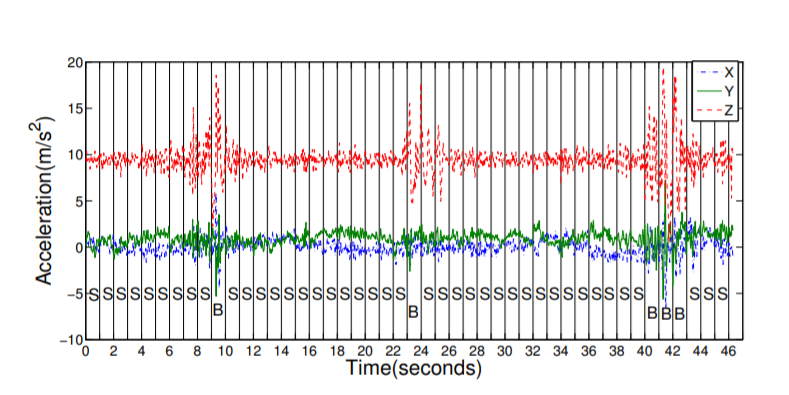
\includegraphics[width=0.75\textwidth]{Images/chapter2/relatedWork1.PNG}
  \caption{Données d'accéléromètre pour trois Ralentisseurs.}
  \label{fig:wolverine_1}
\end{figure}

Une fois cet étiquetage manuel terminé, ils auront  un ensemble de points de données étiquetés. Ceux-ci sont ensuite utilisés pour former un classificateur Support Vector Machine. Ce SVM entraîné, à son tour, est utilisé pour classer les points de données qui sont générés pendant la phase de test, et donc pour prédire l'état du véhicule (Figure \ref{fig:wolverine_1}).

Et pour la détection du freinage du véhicule, la technique utilisée est identique à celle de la détection des bosses, avec deux classes aussi étiquetées doux et freinage (smooth 'S', braking 'R') (Figure \ref{fig:wolverine_2}).

\begin{figure}[h!]
  \center
  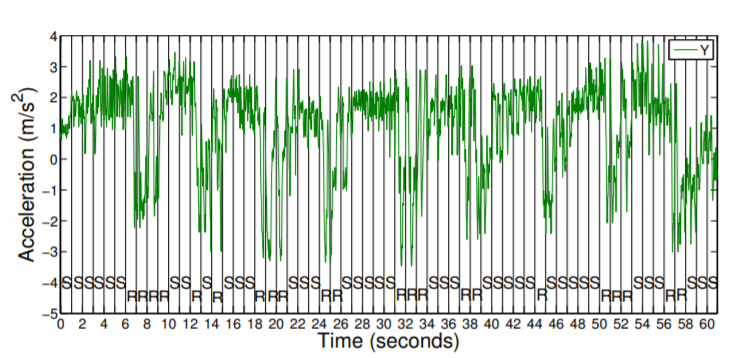
\includegraphics[width=0.75\textwidth]{Images/chapter2/relatedWork2.PNG}
  \caption{Événements de freinage avec étiquettes de classe générées.}
  \label{fig:wolverine_2}
\end{figure}

Ce travail a été fait à Mumbai. L'algorithme identifie correctement 18 des 20 événements de bosse. Aucun tronçon de route lisse n'est identifié à tort comme une bosse. Ainsi, ils obtiennent un taux de faux négatifs de 10\% pour la détection des bosses et un taux de faux négatifs de 21,6\% et un taux de faux positifs de 2,7\% pour la détection de freinage.

\subsection{Real time pothole detection using Android smartphones with accelerometer}
Mednis et al. ont proposé un système de détection des nids-de-poule en temps réel basés sur des données d'accéléromètre pour le déploiement sur des appareils avec des ressources matérielles / logicielles limitées et leur évaluation sur des données du monde réel acquises à l'aide de différents smartphones basés sur Androïd OS.

Ils ont utilisé un dispositif de collier LynxNet modifié \cite{zviedrisLynxNetWildAnimal2010} sur une route avec divers nids-de-poule pour la collecte des données des capteurs de l'accéléromètre.

Après l'acquisition du premier jeu de données de test, une recherche de fonctionnalités liées aux événements potentiels a été effectuée: Le premier et le plus simple algorithme de détection d'événements ZTHRESH a été testé sur l'ensemble des données acquises . Il est similaire à l'algorithme z-peak utilisé dans les systèmes Pothole Patrol \cite{PotholePatrolProceedings}, Nericell \cite{mohanNericellUsingMobile2008}, et limite l'amplitude de l'accélération sur l'axe Z. Les valeurs dépassant des seuls spécifiques sont utilisés pour identifier et classifier les nids de poules (Figure \ref{fig:graph_Z_THRESH}). 

\begin{figure}[h!]
  \center
  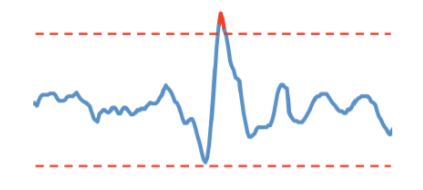
\includegraphics[width=0.75\textwidth]{Images/chapter2/relatedWork3.PNG}
  \caption{Algorithme de détection des nids-de-poule Z-THRESH. Les évènements sont représentés par des mesures avec des valeurs dépassant un seuil spécifié.}
  \label{fig:graph_Z_THRESH}
\end{figure}

Pour la réorientation virtuelle, ils ont utilisé une approche plus simple: un placement contrôlé de l'accéléromètre, éliminant le traitement supplémentaire.

\begin{figure}[h!]
  \center
  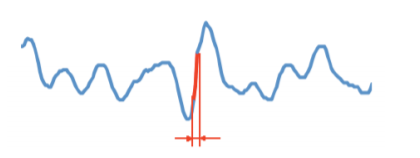
\includegraphics[width=0.9\textwidth]{Images/chapter2/relatedWork4.PNG}
  \caption{Algorithme de détection des nids-de-poule Z-DIFF.}
  \label{fig:graph_Z_DIFF}
\end{figure}

Ensuite, un algorithme légèrement plus avancé était le Z-DIFF (Figure \ref{fig:graph_Z_DIFF}) testé sur l'ensemble de données acquis. Contrairement à Z-THRESH, une recherche de deux mesures consécutives avec une différence entre les valeurs au-dessus du niveau de seuil spécifique a été effectuée. Ainsi, l'algorithme a détecté des changements rapides dans les données d'accélération verticale. L'algorithme nécessite la détermination de la position de l'axe Z de manière similaire à l'approche précédente. 


Les auteurs ont décidé de mettre en œuvre certaines des techniques utilisées pour le post-traitement. Une technique prometteuse pour la mise en œuvre sur un appareil à ressources limitées utilisait un écart type de l'accélération de l'axe vertical. Il a été implémenté dans l'algorithme STDEV (Z) (Figure \ref{fig:graph_STDEV_z}).

\begin{figure}[h!]
  \center
  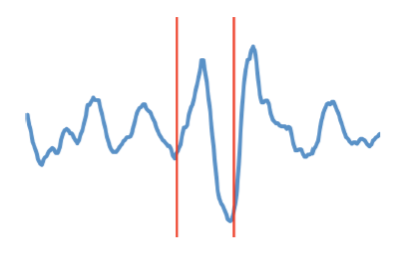
\includegraphics[width=0.85\textwidth]{Images/chapter2/relatedWork5.PNG}
  \caption{Algorithme de détection des nids-de-poule STDEV(Z).}
  \label{fig:graph_STDEV_z}
\end{figure}

En utilisant des outils d'analyse visuelle des données et en recherchant des modèles de données spécifiques, les auteurs ont constaté qu'il existait certains événements caractérisés par un tuple de mesure spécifique. Toutes les données à trois axes de ce tuple avaient des valeurs proches de 0g. ils ont donc nommé cet algorithme G-ZERO (Figure \ref{fig:graph_g_zero}).

\begin{figure}[h!]
  \center
  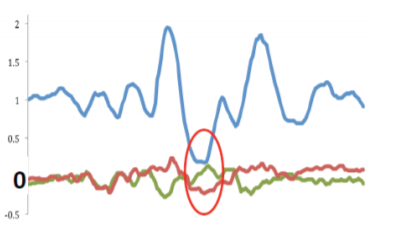
\includegraphics[width=0.7\textwidth]{Images/chapter2/relatedWork6.PNG}
  \caption{Algorithme de détection des nids-de-poule G-ZERO.}
  \label{fig:graph_g_zero}
\end{figure}

\bigbreak
Les algorithmes (Z-THRESH., Z-DIFF, STDEV(Z) et G-ZERO) ont détecté des irrégularités sur la route principale pour 100\% des grands nids-de-poule et 83 à 90\% des grappes de nids-de-poule. Selon l'algorithme, 78 à 89\% pour les petits nids-de-poule ont été détectés. Il est à noter que 9 d'entre eux (50\%) ont été détectés par les 4 algorithmes pour chacune des 10 sessions d'essai sur la route.

En gros, les tests d'évaluation ont abouti à une configuration optimale pour chaque algorithme sélectionné et l'analyse des performances dans le contexte de différentes classes d'irrégularité routière montre des taux de vrais positifs pouvant atteindre 90\%.

\bigbreak
\newpage
Notre algorithme pour la détection de l'état de la route se distingue des travaux connexes de plusieurs côtés:
\begin{itemize}
  \item Nous ne détectons pas d'anomalies spécifiques, par contre nous concluons une évaluation de l'état de la route en général.
  \item Notre solution sera plus simple en utilisant des ressources matérielles et logicielles limitées.
  \item Nous visons à réaliser un prototype rapide, en nous assurant que le système et algorithmes soient extensibles ou facilement remplaçables à tout moment pour des améliorations dans le futur.
\end{itemize}


\begin{table}[]
    \centering
    \begin{tabular}{|m{0.25\linewidth}|m{0.4\linewidth}|m{0.35\linewidth}|}
        \hline
        Parameters                                         & Wolverine                                                        & Mednis                                                   \\
        \hline
        Capteurs                                           & Accelerometre, Magnetometre, GPS                                 & Accelerometre, GPS                                       \\
        \hline
        Methodse pour la reorientation                     & Reorientation utilisant magnetometre et GPS bearing              & Non défini                                               \\
        \hline
        Valeur / Axes pris en compte                       & Z-axis Stdev sur une fenêtre de 1 sec du l'accéléromètre         & Valeurs de l'axe Z de l'accéléromètre                    \\
        \hline
        Techniques utilisées                               & Machine Learning utilisé pour détecter les bosses et le freinage & Z-Thresh, ZDiff, STDEV, G-Zero                           \\
        \hline
        Taux d'échantillonnage réel de l'accéléromètre     & 50                                                               & 100                                                      \\
        \hline
        Lieu d'expérimentation                             & IIT Bombay Campus                                                & Vairoga iela, Riga, Latvia                               \\
        \hline
        Taux d'échantillonnage pris en compte par seconde  & 50 valeurs                                                        & 100 valeurs                                               \\
        \hline
        Équipement utilisé pour la collecte de données     & Capteurs de smartphone (Google Nexus S, HTC Wildfire S)          & Samsung i5700 Samsung Galaxy S HTC Desire HTC HD2        \\
        \hline
        Véhicules utilisés                                 & Suzuki Access 125, Autorickshaw                                  & BMW 323 Touring (4-Wheeler)                              \\
        \hline
        Distance parcourue (km) / temps de trajet (heures) & Non reporté                                                      & 174 KM / Quelques semaines                               \\
        \hline
        Points de montage                                  & Non défini (placé dans une certaine orientation arbitraire)      & Tableau de bord avant                                    \\
        \hline
        Objectif de la détection                           & Bosses, freinage                                                 & Nids de poule                                            \\
        \hline
        Seuil 'threshold' utilisé                          & Non reporté                                                      & Z-Thresh = 0.4g Z-Diff = 0.2g STDEV = 0.2g G-Zero = 0.8g \\
        \hline
        Output                                             & FN - 10\% (2 roues) FP - 8\% (3 roues)                           & 90\% des vrais positifs                                  \\
        \hline
        Consommation d'énergie                             & Consomme 58\% moins d'énergie que Nericel                        & Non reporté                                              \\
        \hline
    \end{tabular} %

    \caption{Comparaison technique des travaux existants.}
    \label{tab:my-table}
\end{table}



\newpage
\section{L'acquisition des données}
Notre système dépend de l'accéléromètre du smartphone attaché à un véhicule, produisant des résultats pour une condition de route donnée et sur la localisation précise de ces résultats à partir du GPS de ce smartphone.
Dans cette section, nous décrivons quelques expériences effectuées par Pothole Patrol \cite{erikssonPotholePatrolUsing2008a} pour valider le fonctionnement des capteurs d'un smartphone et la meilleure position où l'attacher.

\subsection{Positionnement du smartphone}
Une préoccupation est que le placement du smartphone à l'intérieur du véhicule pourrait affecter la qualité du signal de l'accéléromètre. Pothole Patrol ont placé leurs accéléromètres à deux endroits à l'intérieur de la cabine d'une seule voiture. La (Figure \ref{fig:smartphonePosition}) montre le signal de l'accéléromètre pour un tronçon fixe de chaussée à partir de deux positions de montage différentes: fixé au tableau de bord, et fixé sur le côté droit du pare-brise. Les signaux du tableau de bord et du pare-brise semblent assez similaires. 

\begin{figure}[h!]
  \center
  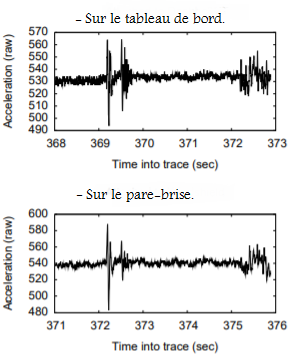
\includegraphics[width=0.50\textwidth]{Images/chapter2/positionmnt.PNG}
  \caption{Comment le signal de l'accéléromètre (axe z) varie avec le placement à l'intérieur de la voiture selon Pothole Patrol.}
  \label{fig:smartphonePosition}
\end{figure}

Ainsi, ils ont fermement fixé l'accéléromètre au tableau de bord à l'intérieur de la boîte à gants de la voiture, qui est un endroit relativement facile pour installer des capteurs et qui les maintient hors de portée des passagers dans la cabine. Il en va de même pour les smartphones.


\subsection{Méthode de récolte de données}
Pour la collecte de données, nous avons créé une application mobile qui utilise les capteurs du smartphone. Principalement l'accéléromètre et le GPS, ainsi que la vitesse du véhicule et des données d'autres capteurs tels que le capteur gyroscopique.

Ceci sera discuté dans la section \ref{sec:app_record}.

\section{Notre Approche}
\label{sec:approache}
Notre approche utilisera principalement les données de l'accéléromètre comme entrées (input).
Ce dernier signale l'accélération du véhicule le long des trois axes du capteur. 

L'accélération mesurée comprend à la fois l'accélération physique du véhicule ainsi que celle de la gravité. La  mesure est signalée dans les champs Accel\_X, Accel\_Y et Accel\_Z. 

En s'inspirant des travaux précédemment cités, considérer uniquement l'axe Z du capteur, en respectant le positionnement du téléphone donné, semble être une méthode à la fois simple et qui donne de bons résultats.

Dans cette section, nous décrivons l'algorithme que nous avons développé pour détecter les conditions routières dans un enregistrement de données de capteurs. 

Le problème de l'identification des conditions routières à partir des données de l'accéléromètre est difficile en raison de plusieurs facteurs tels que le comportement du conducteur (virages, dérapages, freinage brusque, conduite très basse, etc.) ou la grande variation et les conditions routières étranges ici en Algérie, donc notre algorithme suit 3 étapes principales:

\subsection{Windows split and Filtering}
Cette étape est divisée en deux parties:
\begin{description}
  \item[Windows split]:  Les données provenant de la partie d’enregistrement varient en taille, ils peuvent être des enregistrements d’une minute de conduite comme cela peut l’être pendant 1 heure de conduite, notre objectif principal de ce système est de détecter l’état de la route tout au long du chemin, et donc on doit savoir l'état de chaque petite partie de la route enregistrée. L’algorithme proposé divise les données en plusieurs intervalles (fenêtres) en fonction de la distance.
  
  On calcule la distance entre le 1er point et le 100 ème, en utilisant la longitude et la latitude de chacun, si la distance calculée est comprise entre 90 et 110 mètres on va utiliser cette fenêtre, sinon on augmente ou diminue l'intervalle de points choisi.

  Pour faire cela nous avons utilisé la formule de Haversine \cite{HaversineFormula2020}:

  Nous convertissons d'abord le long et le lat de chaque point en radians:

  Valeur de la latitude en radians, \[lat = Latitude / (180/\pi)\]

  Valeur de la longitude en radians, \[long = Longitude / (180/\pi)\] 


  Ensuite, pour obtenir la distance entre le point A et le point B, nous utilisons la formule suivante:

   \[
    d = radius   \cdot \arccos
    \left[
        \left(
            \sin(lat_{A}) \cdot \sin(lat_{B})
        \right)
        + 
        \left(
            \cos(lat_{A}) \cdot \cos(lat_{B}) \cdot \cos(long_{B} - long_{A})
        \right)
        \right]
\]
Tel que : 
\begin{itemize}
  \item[$\ast$] $radius  = 6371 * 10^{3} $ m.
  \item[$\ast$] d est la distance obtenue en mètres.
\end{itemize}
 
\item[Speed filtering]: Une fois les données divisées en fenêtres, nous devons filtrer les fenêtres inutiles avant le traitement. 

Dans cette partie, nous filtrons chaque fenêtre  selon la vitesse du véhicule. Les fenêtre dans lesquelles le véhicule ne se déplace pas ou se déplace très lentement sont ignorées (nous avons utilisé 20 km/h comme seuil de vitesse).

\end{description}


\begin{figure}[h!]
  \center
  \begin{subfigure}{.75\textwidth}
      \center
      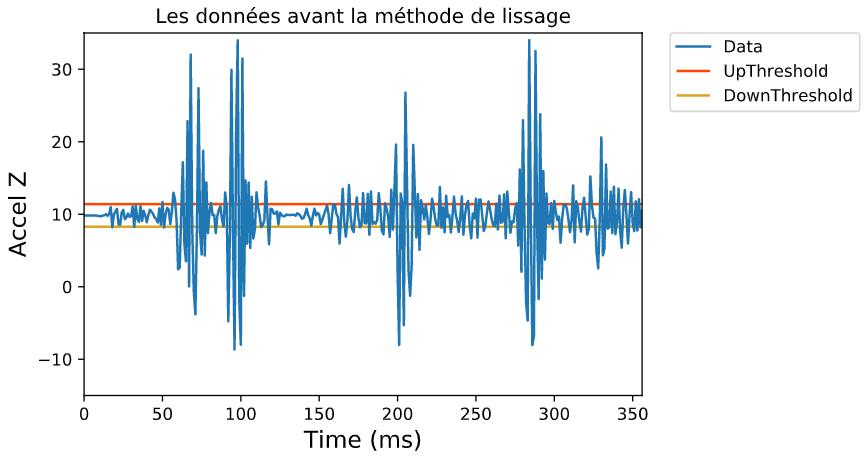
\includegraphics[width=0.8\textwidth]{Images/chapter2/approache/avantissage.png}
      \caption{Les données avant la méthode de lissage.}
      \label{fig:avantlissage}
  \end{subfigure}
  \begin{subfigure}{.75\textwidth}
      \center
      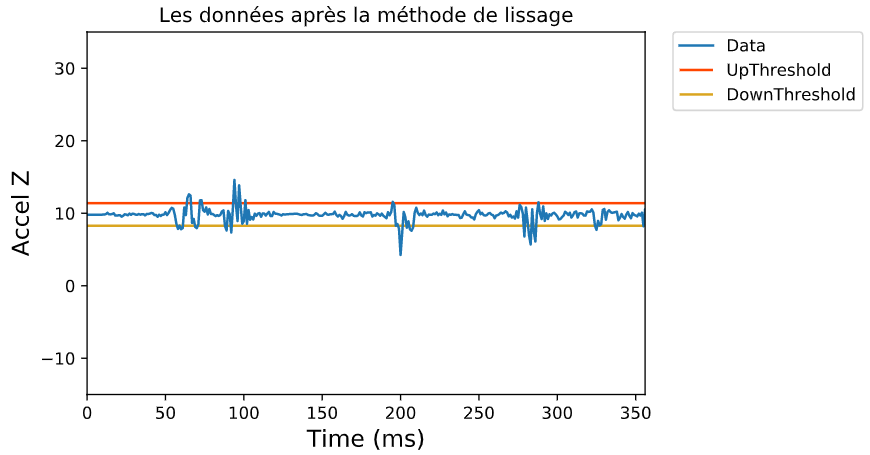
\includegraphics[width=0.8\textwidth]{Images/chapter2/approache/apreslissage.png}
      \caption{Les données après la méthode de lissage.}
      \label{fig:apreslissage}
  \end{subfigure}
 
  \caption{Le lissage des données.}
  \label{fig:lissage}
\end{figure}

\subsection{Lissage et valeur des seuils}
Une fois que l’algorithme a obtenu les données filtrées, il commence par les lisser pour éliminer les vibrations normales, puis calcule la valeur moyenne de toutes les données afin de l’utiliser comme référence pour détecter les valeurs anormales.

La méthode de lissage que nous avons utilisée consiste à remplacer chaque point par la moyenne de ce dernier avec les 2 valeurs avant et après chaque point concerné. 

Le moment où la valeur moyenne est calculée  et en se basant sur notre état de l'art [\ref{tavauxconnexes}], et quelques tests sur des données réels nous avons choisi 0,85 g comme valeur de sensibilité afin de calculer le seuil (Figure  \ref{fig:lissage}).

Nous avons calculé les valeurs de seuil comme suit:

\[UpThreshold = Average   * SensitivityValue\]

\[DownThreshold =  Average  * 1/SensitivityValue\]

  Tel que:
  
\begin{itemize}
  \item[$\ast$] UpThreshold : Valeur du seul supérieur.
  \item[$\ast$] DownThreshold : Valeur du seul inférieur.
  \item[$\ast$] Average : La valeur moyenne de toutes les données de la fenêtre.
  \item[$\ast$] SensitivityValue: 0.85 g.
\end{itemize}


\subsection{Z Score}
Une fois les données prêtes à être traitées, et que les valeurs des seuils sont calculées. On s’intéresse aux points dépassant ces valeurs de seuil qui représentent probablement des anomalies dans la route.

On compte ces valeurs pour calculer le score de qualité de ce morceau  de route.




\begin{figure}[h!]
  \center
  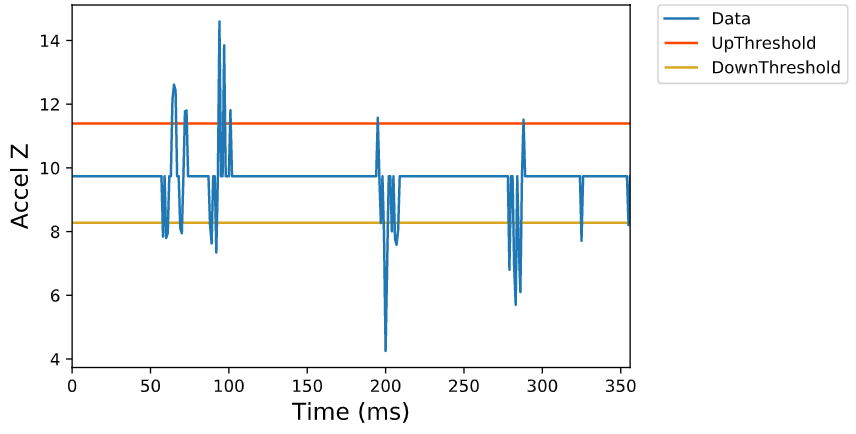
\includegraphics[width=0.85\textwidth]{Images/chapter2/approache/zscore.PNG}
  \caption{Les données  dépassant les valeurs de seuil.}
  \label{fig:zscore}
\end{figure}

Nous appelons ce score le Z Score, c'est une valeur entre 0 et 1 ( 0\% à 100\%), plus la valeur est élevée, plus la route est de mauvaise qualité.